\chapter{Backlog}

\begin{figure}[h]
    \centering
    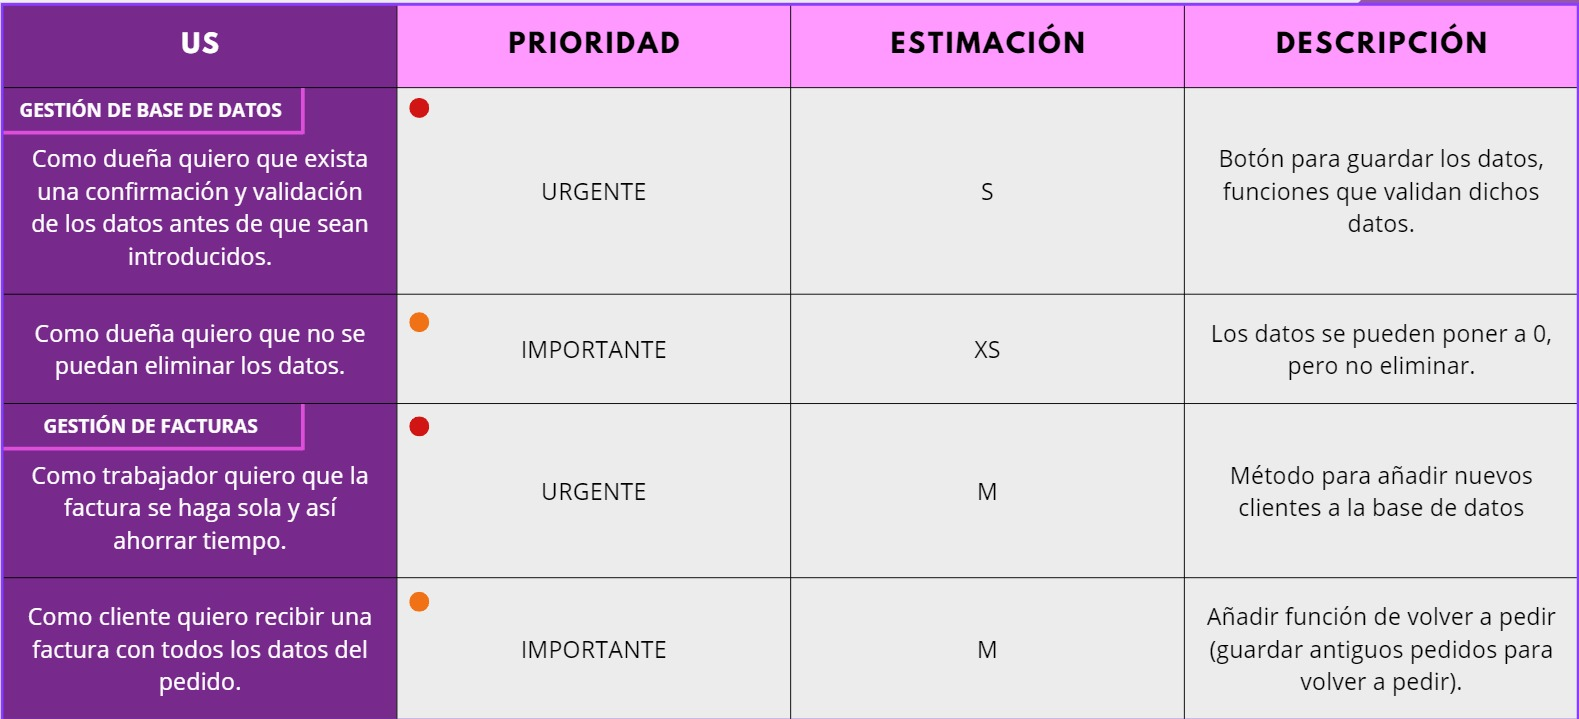
\includegraphics[width=1\textwidth]{figures/backlog-1.jpeg}
    \caption{Primera parte del Backlog}
    \label{fig:backlog1}
\end{figure}

\begin{figure}[h]
    \centering
    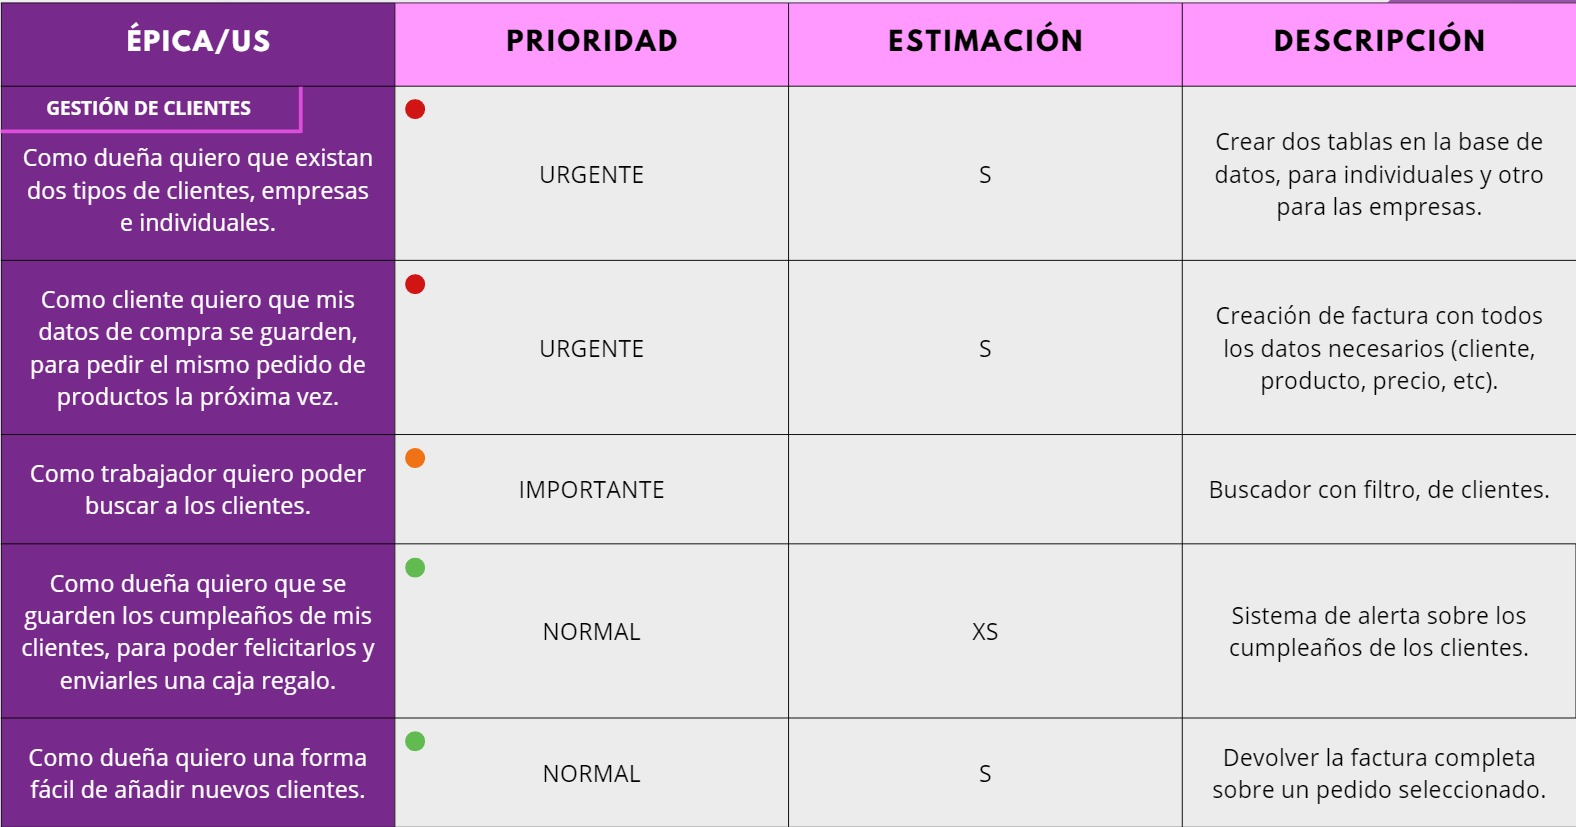
\includegraphics[width=1\textwidth]{figures/backlog-2.jpeg}
    \caption{Segunda parte del Backlog}
    \label{fig:backlog2}
\end{figure}

\begin{figure}[h]
    \centering
    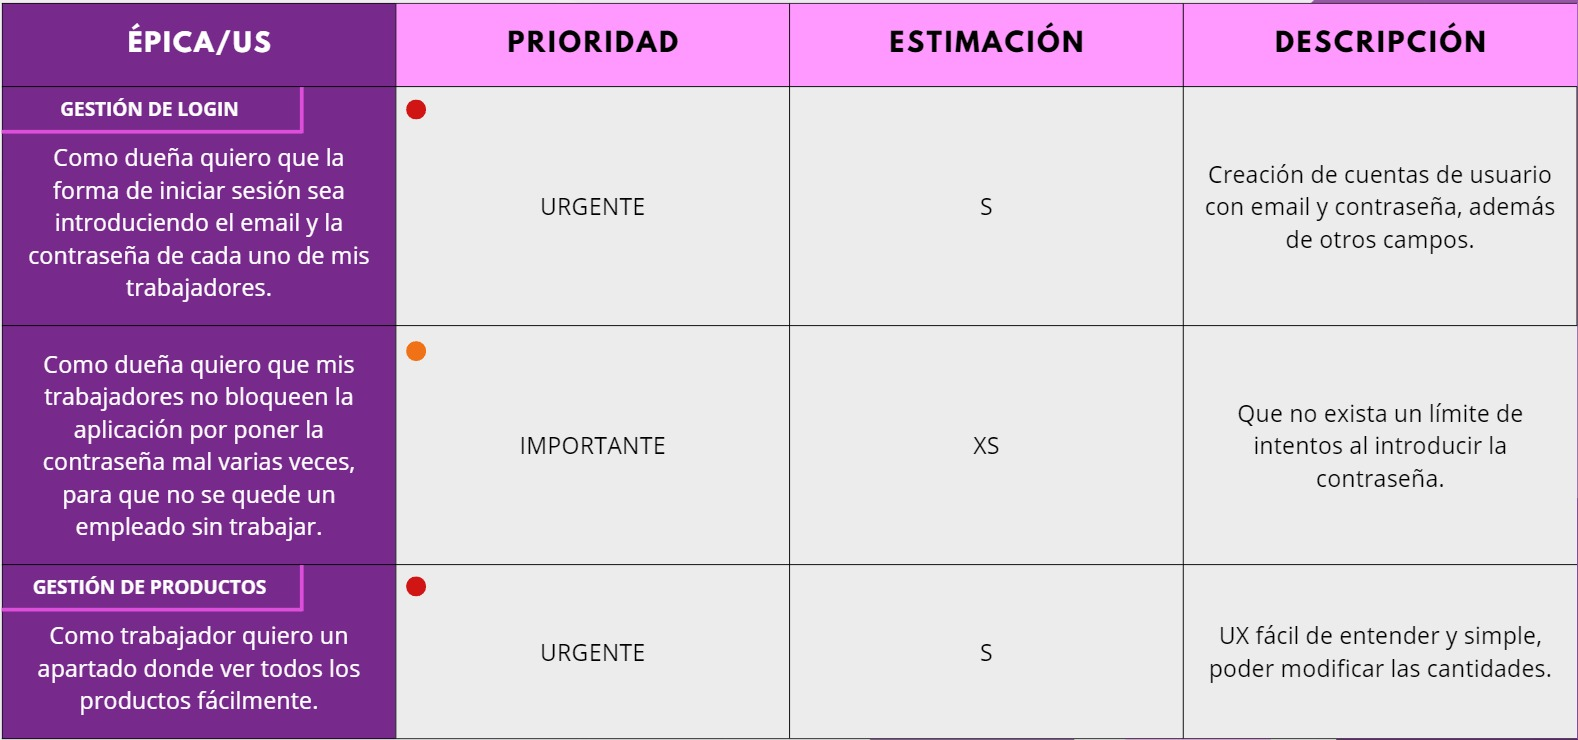
\includegraphics[width=1\textwidth]{figures/backlog-3.jpeg}
    \caption{Tercera parte del backlog}
    \label{fig:backlog3}
\end{figure}

\begin{figure}[h]
    \centering
    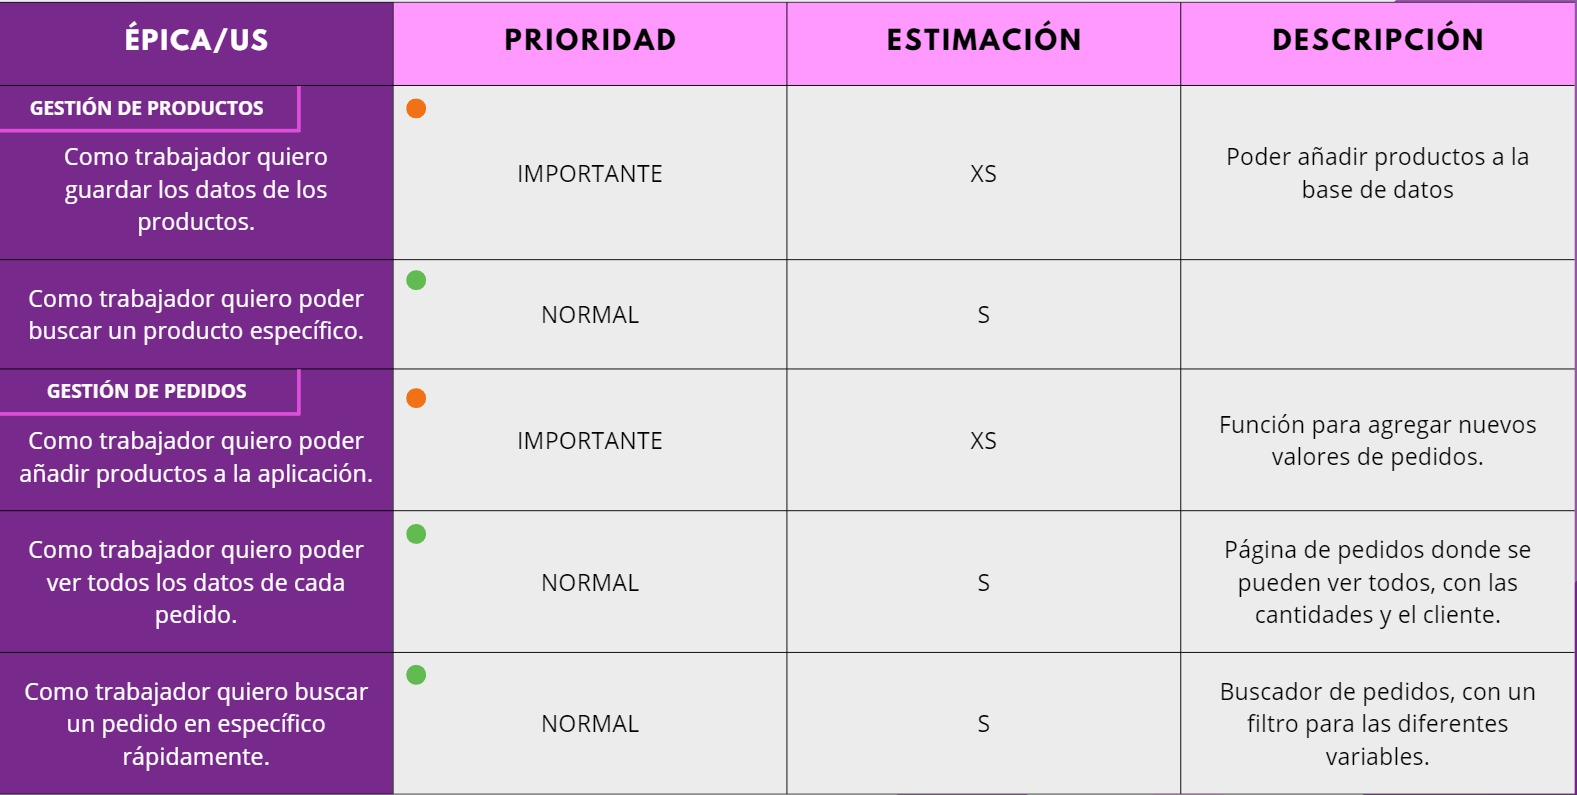
\includegraphics[width=1\textwidth]{figures/backlog-4.jpeg}
    \caption{Cuarta parte del Backlog}
    \label{fig:backlog4}
\end{figure}

\begin{figure}[h]
    \centering
    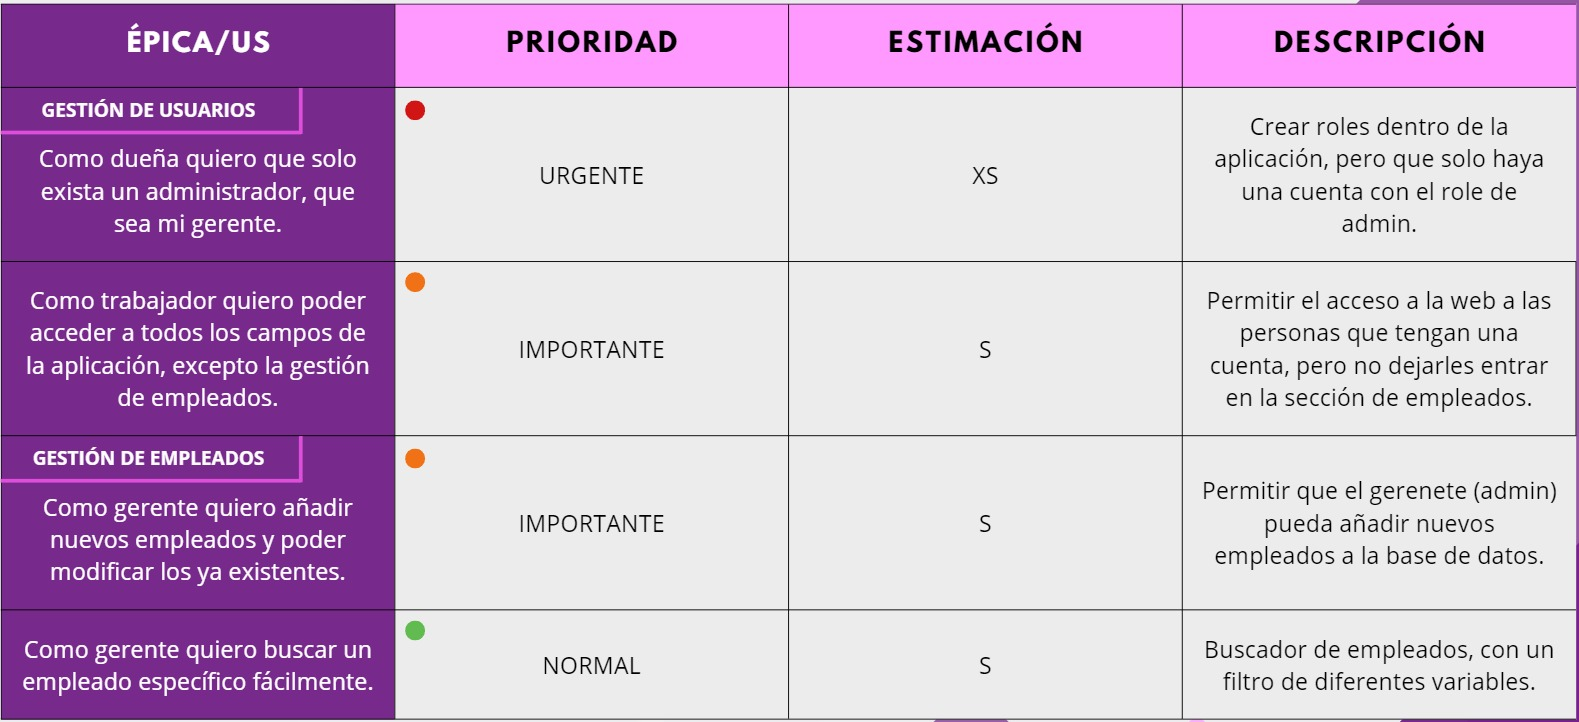
\includegraphics[width=1\textwidth]{figures/backlog-5.jpeg}
    \caption{Quinta parte del Backlog}
    \label{fig:backlog5}
\end{figure}
